\chapter{Simulation}

The frontend can be quite interesting as just a way to survey a city from a bird's eye view. The program's real use lies in data analysis, though, as the task description suggests. Over the semester, I tried multiple approaches for creating an agent-based simulation, with all but the last attempt failing due to technical circumstances. The final implementation is a simple but effective model heavily reliant on the software's backend with the frontend only serving as a visualisation tool.

\section{Deprecated versions}

The first concept was very simple. Each agent would pick a random building to start at and head to in a straight line, with a constant speed. Each agent would be shown in the graphical scene, and the visuals would not be unlike an ant colony. The backend simulated movement in one minute steps, and after each one, the modified agents would be collected and sent over the websocket in a few chunks, so as to reduce the chances of the socket crashing. The problem here was one of scalability. Fifty or a hundred agents could easily be processed and shown in real time, but that obviously was not enough to draw any meaningful conclusions about transit behaviour. Displaying more agents caused a simply unacceptable framerate of three frames per second at most. Although I used the same model for every agent, batching and caching could not be used due to the chaotic nature of their overall movement.
%TODO image of orange cubes

The second version improved performance by processing the agent updates non-visually and dividing up the playfield into relatively small chunks to act as a heatmap; it was a separately renderable on top of the main scene. Each update's coordinates were fed into the overlay, and an opacity value was calculated for every chunk. The result was a serviceable tool that, while updating constantly, still had bad performance. A new object cache was being created every time I opened the heatmap UI, and this taxed the rendering thread heavily. However, once all updates have been processed, the performance was decent. This gave me the idea of running full simulations as fast as possible, and only transferring a minimal amount of information over the socket.
\begin{figure}[h]
    \centering
    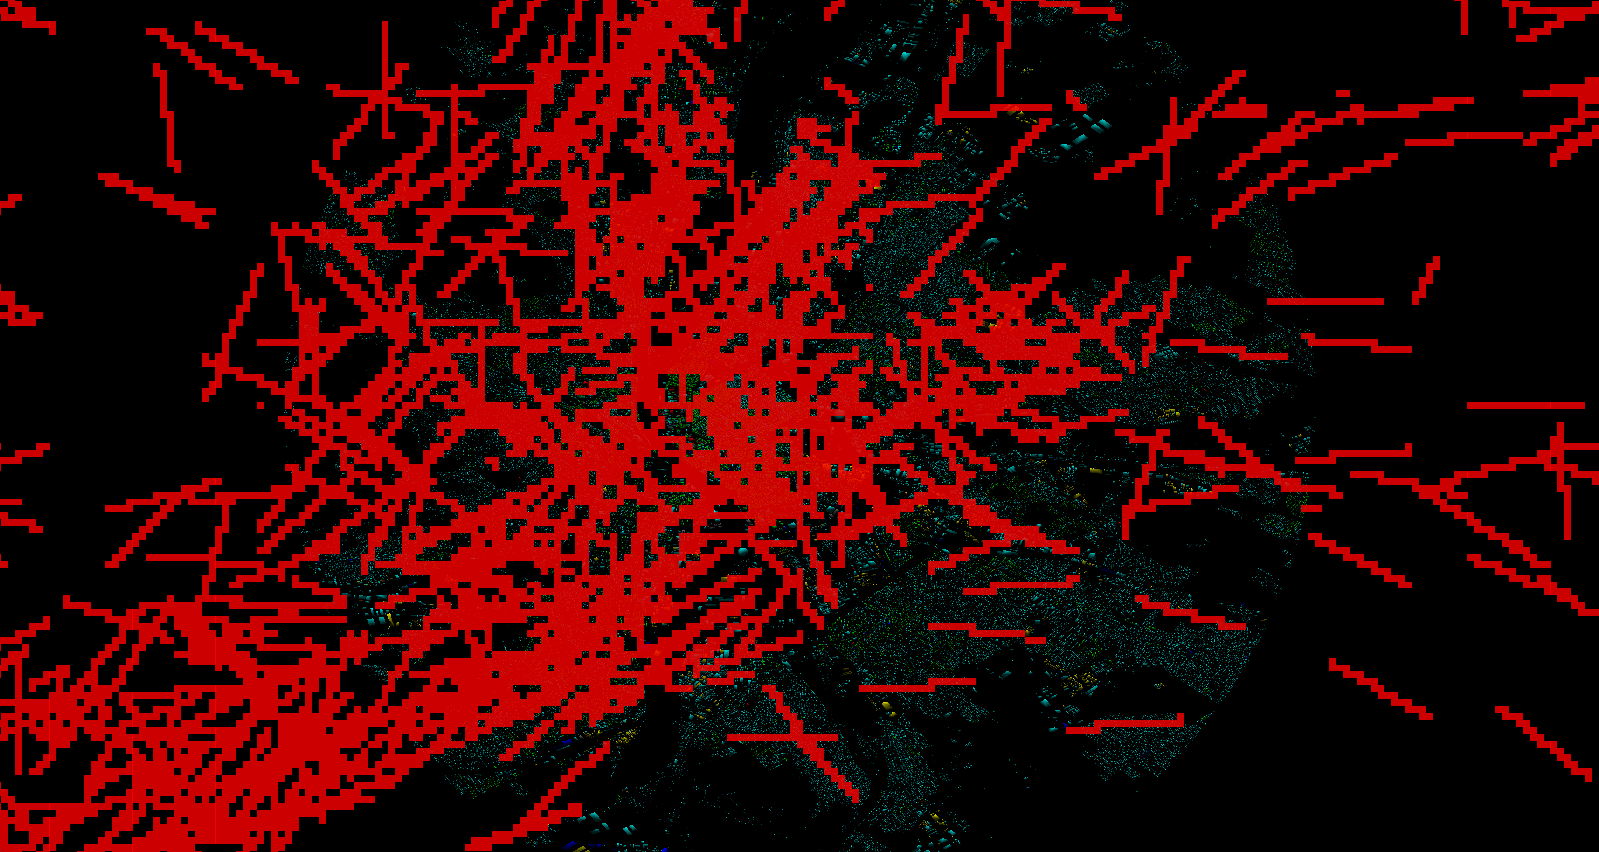
\includegraphics[width=140mm, keepaspectratio]{images/overlay_v2.png}
    \caption{An overlay with flattened opacity, displayed over the city of Budapest. Agent paths are randomised and are traversed in a straight line\ \label{overlay_v2}}
\end{figure}

\section{The working implementation}

